\documentclass[12pt,oneside,a4paper,english]{article}
\usepackage[T1]{fontenc}
\usepackage[utf8]{inputenc} % Changed from latin2 to utf8 for better compatibility
\usepackage[margin=2.25cm,headheight=26pt,includeheadfoot]{geometry}
\usepackage[english]{babel}
\usepackage{listings}
\usepackage{color}
\usepackage{titlesec}
\usepackage{titling}
\usepackage[framed, numbered]{matlab-prettifier}
\usepackage{changepage}
\usepackage{amsmath}
\usepackage{hyperref}
\usepackage{enumitem}
\usepackage{graphicx}
\usepackage{fancyhdr}
\usepackage{lastpage}
\usepackage{caption}
\usepackage{tocloft}
\usepackage{setspace}
\usepackage{multirow}
\usepackage{titling}
\usepackage{float}
\usepackage{comment}
\usepackage[strings]{underscore}
\usepackage{booktabs}
\usepackage{indentfirst}
\usepackage{lscape}
\usepackage{booktabs,caption}
\usepackage[flushleft]{threeparttable}
\usepackage[english]{nomencl}
\usepackage{xcolor}
\usepackage{lipsum}

% Set up hyperref
\hypersetup{
colorlinks=true,
linkcolor=blue,
filecolor=magenta,
urlcolor=cyan,
pdftitle={Review Of Historical Astronomical Tools},
pdfpagemode=FullScreen,
}

% --- set footer and header ---
\pagestyle{fancy}
\author{}
\fancyhf{}
\lhead{Appendix: Observing The Moon}
% --- Title formatting ---
\title{\textbf{Moon Observation Appendix}}
\date{\today}

\begin{document}
\maketitle
\begin{abstract}
    When observing the Moon, there are many properties that can be directly observed and predicted. Many characteristics can be observed from the surface of Earth or very accurately predicted! This document is a supplement to \textit{The Orbital Mechanics and Magnetic Characteristics of The Moon}.
\end{abstract}
\section{Measuring The Position and Orbital Velocity of The Moon}
Using the Lunar Laser Ranging(LLR) Experiment, we can find the current position of the Moon and predict where the Moon will be. So, NASA runs the LLR; this experiment uses mirrors placed on the Moon by Apollo(USA) and Luna(USSR) Astronauts in the 1970s, LLR uses these retroreflectors to measure the distance of the Moon is from the Earth. 
\begin{figure}[H]
    \centering
    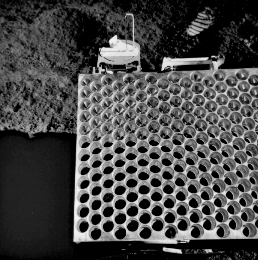
\includegraphics[width=0.4\textwidth]{Reflector.png}
    \caption{Apollo 15 retroreflector. \cite{apolloretro}}
    \label{fig:apolloretro}
\end{figure}
The technology used is known as LIDAR. The principle is inherently simple, light travels at a constant velocity $c$. The retroreflectors are specialized mirrors to reflect the incoming light directly back from the direction it hit the mirror. The principle equation is:
\begin{equation}
    d=\frac{c*\Delta t}{2}
\end{equation}
The distance is simple the time it takes to travel to and from the reflectors($\Delta t$). This experiment is still a challenge, most photons sent are lost or not reflected back at the observing telescope. By using Monochromatic light(Light of a specific wavelength). Many scientific and governmental bodies use these retroreflectors, to find the distance to the Earth from the Moon. The Experiment is not something an amateur can do! The experiment requires a high powered lasers like Apache Point Observatory Lunar Laser Ranging Operation(\href{https://tmurphy.physics.ucsd.edu/apollo/apparatus.html}{APOLLO}). 
\subsection{Measurement and Prediction of the Moons Distance}
The Moon's orbit and location are very well understood, so we can predict the Moon's location and it's distance from Earth accurately. Using EUROLAS Data Center (EDC) data browser we can search for OPAs(predictions)
\begin{figure}[H]
    \centering
    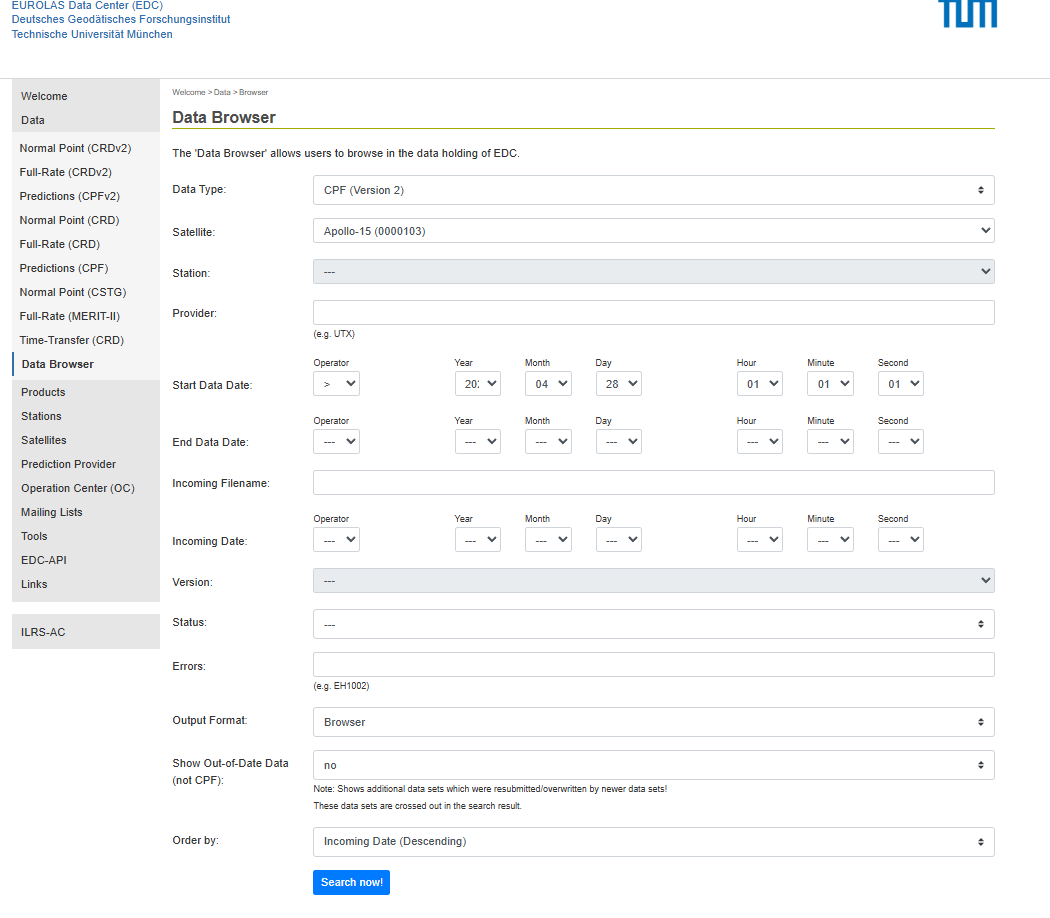
\includegraphics[width=0.7\textwidth]{EDC1.png}
    \caption{Search Apollo15 and Data Type CPF2 for the Apollo 15 reflector on the Moon at \href{https://edc.dgfi.tum.de/en/data/browser/}{EDC Data Browser}.}
\end{figure}
One line of this data table will be:
\begin{itemize}
    \item[] 10 1 60794       0.0 0      -315941963.394       -85456968.567       143416091.775 
    \item[] 10 2 60794       0.0 0       315952958.458        85468954.116      -143438183.860 
    \item[] 30 1        1928.     -33457.      11046.    23.7 
    \item[] 10 1 60794     900.0 0      -320591682.743       -65457738.637       143685862.688
\end{itemize}
Each item is seperated by whitespace, rows with the record 10 are what is important. Each 1 whitespace character after 10 seperated mean:
\begin{itemize}
    \item Direction Flag(I1) - Either 0,1,2(-1 = Error), this flag defines if the cooridinates are viewed from Earth or the Moon. Note how the signs are flipped
    \item Modified Julian Date (MJD)(I5) - Julian date(Use online converter) is simply counting the progression of dates starting from 1873BC, used by astronomers. Modified Julian Date is the original julian date is $MJD = JD - 2400000.5$, Apr 29, 2025 MJD is 60794.
    \item Seconds of Day (UTC) - The time of measurement in the day of the MJD.
    \item Geocentric X - Geocentric 3D X cooridinate of Moon's distance in meters.
    \item Geocentric Y - Geocentric 3D Y cooridinate of Moon's distance in meters.
    \item Geocentric X - Geocentric 3D Z cooridinate of Moon's distance in meters.
\end{itemize}
From the \href{https://ilrs.gsfc.nasa.gov/docs/2018/cpf_2.00h-1.pdf}{\textit{Consolidated Laser Ranging Prediction Format}} shared by NASA in 2018. It's noted that: 
\begin{quotation}
    Record pairs like position(10), directions 1 and 2, and corrections 30, directions 1 and 2 should be treated as a single-time set of predictions.
\end{quotation}
For the sake of simplicity we will ignore the correction rows. The location of the Moon is given in geocentric cooridinates in 3D(X,Y,Z). To find the radius or distance to the Moon is found with a simple equation:
\begin{equation}
    R = \sqrt{X^2+Y^2+Z^2} 
\end{equation}
\begin{equation}
    = \sqrt{315941963.394^2+(-85456968.567)^2+143416091.775^2} = 357337925.625
\end{equation}
Meaning based on the first row, the moon is 357337925.625 meters or 357337.92562 kilometers from the Earth. Take the average of the 2 time=0.0 0 rows make the Moon's mean radius on April 29th, at Midnight(UTC) is 357348652.946 meters or approximately 357348 kilometers. The time between prediction intervals are 900s apart 15 minutes. Unfortunately, NASA is modifying their data centers and data products, so there is no observational data availible recently from the LLR experiment. prediction data is availible to be used and can be understood to be mostly correct for tracking purposes. The orbital velocity of the Moon can be determined by simply:
\begin{equation}
    v_{Moon} = \frac{r_2-r_1}{t_2-t_1}
\end{equation}
Currently, there is no clear timeline on when measured data will be published from the various LLR data past April 8th, 2025.
\section{Moon's Temperature}
When it comes to measuring the temperature of the Moon, the temperature on the surface of the Moon, fluctuates from 127 Degrees Celsius and -173 Degree Celsius depending if the surface is facing the Sun. The temperature of the Moon is recorded with NASA's Lunar Reconnaissance Orbiter(LRO) with the DIVINER Lunar Radiometer Experiment. This is an infared thermometer like consumers use. The author implores the reader to understand that there is no weather on the Moon, the temperature on the Moon's surface depends on it's distance from the Sun. Unfortunately, Diviner is not sharing live public science data. There is no way to get live measurements of the Moon's whole surface temperature live. There are temperature maps taken over a few hours while the LRO orbits the Moon collecting temperatures across the surface. 

\section{Albedo, Brightness, Luminosity and Magnitude}
\subsection{Brightness \& Luminosity}
The Albedo, Brightness and Luminosity are closely relatred concepts. Talking about one without the others is not a completely proper explantion. The first question is what the brightest object in the sky? What's the brightest object in the galaxy? Obviously, the sun is the brightest thing astronomers observed. Astronomers of yore used a seemingly random scale, simply counting the number for stars in the sky of a certain "magnitude" of brightness. Brightness is known by astronomers as magnitude, this depends on the celestial body's Luminosity, distance and factors that could dim the light coming to the observer on Earth(known in general as Extinction). 

Lumninosity is intrinsic and is a measure of the electromagnetic flux per unit area from it's surface, its units are watts per square meter. Magnitude of brightness can be either apparent magnitude or absolute magnitude, apparent depends on the observer's location, while absolute predicts its brightness without any effects from extinction from a standard distance away. The last and important characteristc is Albedo, Albedo is a measure of how reflective a body or item is, everything from tomatoes to the Moon has Albedo! Albedo is an intrinsic property of planets in our solar system, planets and the Moon don't have luminosity because its not emitting light, but they do have brightness! The apparent magnitude(brightness) is based on the Albedo of the Moon.

\subsection{Apparent Magnitude}
The apparent magnitude depends on the band of light you're observing. For the Moon, we use the visual band as the light reflected from the Moon is mostly in the visual band. In the past, astronomers calibrated brightness based off a certain star. In the past Vega was used, and their brightness(photon flux) is compared to Vega. The Sun's apparent magnitude is -26.832. This is calculated via the following:
\begin{equation}
    m = -2.5 *log_{10}(\frac{F_x}{F_{x,0}})
\end{equation}
Where $F_x$ is the measure of electromagnetic or photon flux in spectrum you're observing. We will assume the visual band, $F_{x,0}$ is the "zero" flux, or a calibrating point, historically based on Vega.
\subsubsection{Magnitude vs Luminosity}
Considering the Sun's Luminosity, we can compare that to the magnitude that we observe on the Earth's surface, not all of the light emitted from the Sun hits the Earth, some of the light is absorbed by our atmosphere and some is reflected too. Lumninosity is intrinsic to all stars. Apparent Magnitude is the brightness of the Sun or body from the Earth, it is literally the apparent brightness observed, a value that is between these two values is the absolute magnitude. This attempts to place every star or body at the same distance from the observer. In our solar system, astronomers use 1AU(Earth-Sun Distance) or 10 parsec(32.6 Lightyears) for sources outside of the solar system. This is a calculated measurement, that is not as important for the reader to know as it depends on a very complicated model and is being improved by astronomers \textbf{Apparent magnitude measurement at the V-band(visual band), are centered at 551nm which roughly aligns with brightness percieved by the human eye.}
\subsubsection{Sample Calculation}
We can calculate the Sun's Apparent Magnitude using the Sun's flux in the V-band, in this calculation: we will use the non-SI unit, Jansky's which is flux but centered at a specific wavelength, generally this also more closely aligned with how data will come from photometry equipment. Using the zero point flux of $F_{x,0}$=3640 Janksys.\cite{metrics} Meawhile the Sun's flux in the visual band is 1.803$\cdot10^{14}$ Janksys
\begin{equation}
    m = -2.5 *log_{10}(\frac{1.803\cdot10^{14}}{3640})
\end{equation}
\begin{equation}
    m = -2.5 *log_{10}(4.95\cdot10^{10}) = -2.5(10.69) = -26.74
\end{equation}
The Sun's apparent magnitude, is negative because the scale is logarithmic, negative means this object is object is very bright and there is less of this object in the sky, positive apparent magnitude things like stars are plenty, while there are only a few bodies comparitively that are negative(planets and moons). The Moon has an apparent magnitude of anywhere from -12 to -4 apparent magnitude. The apparent magnitude is 400,000 times less than the Sun. The apparent magnitude depends on many things like the literal distance from the Moon or the amount of the lit Moon is visible to the observer. Without doing too much mathematics, The reader can also, just compare the astrocamera flux in the daytime vs when pointed at the Moon, the apparent magnitude is just a ratio of brightness.

Using JPL's Horizon system, you can see the upcoming apparent brightness of the Moon(\href{https://ssd.jpl.nasa.gov/horizons/app.html#/}{JPL Horizons System}).
\begin{figure}[H]
    \centering
    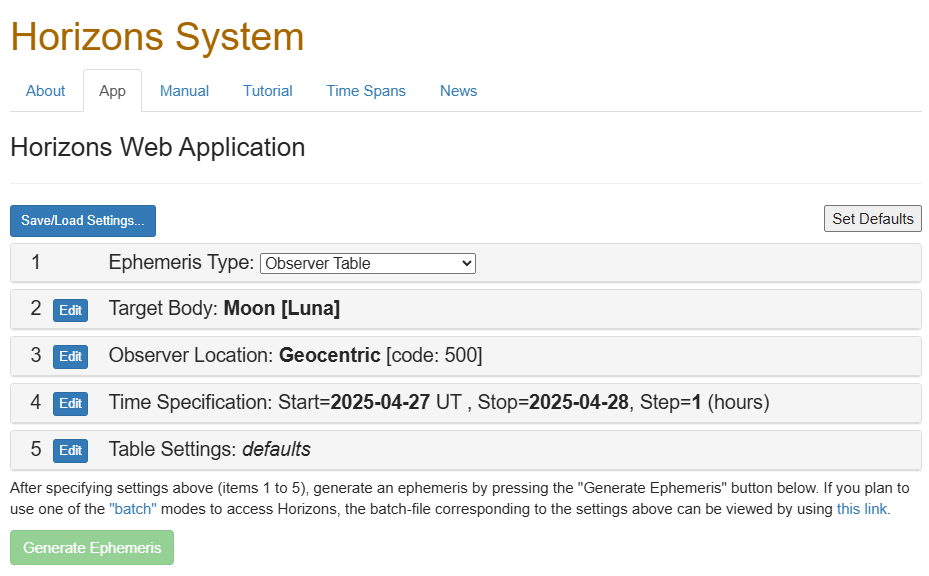
\includegraphics[width=0.7\textwidth]{HorizonJPL.png}
    \caption{Sample search for information, generate Emphemeris and search for APmag to see hourly results at JPL Horizons System}
\end{figure} 
The brightness have many practical challenges to measurement like atmospheric scattering and scattered light due to dust in the solar system. As noted, when reading the data key. The magnitude is .12 lower than what was expected due to Extinction from atmospheric scattering. If you want to verify the apparent magnitude, you can use an Astrocamera(check \href{https://www.aavso.org/ccd-camera-photometry-guide}{AAVSO's CMOS Photometry Guide} for links on where to get them).

\subsection{Albedo}
Since the Moon doesn't produce any of it's light, all of its light is reflected. This is based on the brightness of the Moon observed, planets like Venus have a very high albedo becuase it's atmosphere is full of reflective gases, Venus has an albedo of .7. The Moon is mostly comprised of volcanic rock and has no atmosphere, which means it will have a significantly lower albedo. As with apparent and absolute magnitude, Bond Albedo exists to describe an absolute albedo regardless of the angle of the Moon to the Sun vs the observer viewing it. Bond Albedo accounts for all wavelengths of light and all phase angles, \textbf{Bond albedo can ONLY be measured from space. The Lunar Reconnaissance Orbiter(LRO), has measured the bond albedo of .12, This value doesn't change as the Moon orbits the Earth.}

\section{Other Values}
\textbf{The Moon doesn't have Entropy or a Magnetic Field Vector}. Firstly, entropy is a measure of the number of identical states in a thermodynamic system, this is also known as a measure of chaos in the system. Meanwhile, magnetic fields are describe with vectors, the Moon has trace magnetic fields on its surface from ferromagnetic materials leftover from asteroids and the Moon's past active core. 
\newpage
\section{References}
\bibliography{OrbitalMech.bib}
\bibliographystyle{ieeetr}
\end{document}


